%!TEX root = doc.tex
\section{The \apiname{} API} % (fold)
\label{sec:proposal}

At times, when developing MAS on a specific platform, a need arises for adopting different tools than those available in the original platform. More specifically, this paper is the result of a necessity to quickly and easily create JADE-based applications out of Repast-based simulations, eventually being able to perform the complementary operation. \apiname{}'s main goal is to enable in Repast the support for the development of FIPA-compliant MABS. In this section we try to give a thorough description of \apiname{}'s architecture while comparing our design decisions with those of JADE.
% [citation needed: is conversion a real need?]

\subsection{Repast and JADE}
% What was missing in Repast?
JADE and Repast are two popular agent-based application development tools with a very distinct set of features. Table \ref{tab:jadevsrep} summarizes the main differences between the two. It's worth pointing out that communication and ontologies are both covered by FIPA specifications. This, together with the differences in agent execution, make up the targets of out API.

Our goal is not to reproduce JADE's distribution architecture in Repast. One advantage of using Repast is that, since the communication is local (while JADE's agents are often spread in different containers), the execution of Repast-based simulations is typically much faster. This also makes it more suited to perform simulations and tests on MAS \cite{mengistu2008scalability} \cite{gormer2011jrep} \cite{garcia2011misia}.

By incorporating FIPA specifications in Repast, we bring it closer to JADE. By using \apiname{}, programmers that are already comfortable with creating MAS in JADE can feel comfortable enough to produce Repast-based simulations with the tools they're used to in JADE.

\begin{table}[h]
	\normalsize
	\caption{Summary of JADE and Repast features.}
	\label{tab:jadevsrep}
	\begin{center}
		\begin{tabular}{l|cc}
		\hline

		\hline
		\textbf{} & \textbf{JADE} & \textbf{Repast} \\ %& \textbf{Cougaar} \\
		\hline
			Agent 		& FIPA  	&  Method calls  \\ %& Serialized Object \\
			Interaction	& protocols	&  Shared resources \\
		\hline
			Distribution & Yes & No \\ %& Yes \\
		\hline
			Simulation Tools & No & Yes \\ %& Yes \\
		\hline
			Scalability & Limited & High \\ %& High \\
		\hline
			Ontologies & Yes & No \\ %& Yes\\
		\hline
			Open Source & Yes & Yes \\ %& Yes\\
		\hline
			Agent  		& Behavior-based & Schedule-based  \\ %&  \\
			Execution	& Multi-threaded & Single-threaded \\ %&  \\
						& Event-driven   & Tick-driven 	   \\ %&  \\
						& Assync		 & Sync 		   \\ %&  \\
		\hline
		\end{tabular}
	\end{center}
\end{table} 

\subsection{FIPA Specifications}

As mentioned before, \apiname{} closely follows JADE's architecture regarding the use of protocols and services specified by FIPA. The architecture described in this paper includes four main concepts proposed by FIPA: the Directory Facilitator (DF), the Message Transport Service (MTS), the ACL Message and the Interaction protocols.

The DF is a component that provides a yellow page service and is part FIPA Agent Management Specification \footnote{FIPA AM - http://www.fipa.org/specs/fipa00023/XC00023H.html}. It allows one agent to perform searches in order to request information about other agents. Only agents that are registered in the DF will be indexed and agents can register and deregister themselves at any time. These searches can be filtered in order to find the agents that are announcing themselves as providers or certain service. 

In \apiname{}, the services used as filters in search are the type of interaction behavior that an agent is expected to have adopted. Since the context of out tool is the development local (vs. distributed) simulations, a single DF exists in each simulation. Is worth noting that Repast has it's own agent manager, named ``Context''. \apiname{} offers support to this feature by integrating a reference to this object in the DF.

The MTS is a service, also specified by FIPA \footnote{FIPA MTS - http://www.fipa.org/specs/fipa00067/SC00067F.html}, for transportation of ACL messages between agents. One of its tasks is to be able to resolve agent addresses, in order to be able to deliver those messages. \apiname{}'s implementation of the MTS is simplified. Since \apiname{}'s target is the development of simulations in Repast, all our agents are local and agent address resolution is not required.

The ACL Message is the envelope that contains the details for communication. ACL (Agent Communication Language) is specified by FIPA, which stipulates what fields the message should contain. Table \ref{tab:fipaACLMessage} was adapted from the FIPA ACL Message structure specification and gives and contains the list of fields in a message. Not all of them are mandatory. FIPA specifies the \texttt{performative} as the only mandatory field, although the \texttt{sender}, \texttt{receiver} and \texttt{content} are usually expected to be present.\footnote{http://www.fipa.org/specs/fipa00061/SC00061G.html}.

Our implementation uses a version of the ACL Message that is slightly simpler than in the one found in JADE. The language, encoding and reply-by fields were omitted in the current version. Also, the ontology field is simply a text field. \apiname{} does not support more complex ontologies at present time.

\begin{table}[h]
	\normalsize
	\caption{FIPA ACL Message Parameters}
	\label{tab:fipaACLMessage}
	\begin{center}
		\begin{tabular}{cc}
		\hline
		\textbf{Parameter} & \textbf{Category of Parameters} \\
		\hline
		\texttt{performative} & Type of communicative acts \\
		\hline
		\texttt{sender} & Participant in communication \\
		\hline
		\texttt{receiver} & Participant in communication \\
		\hline
		\texttt{reply-to} & Participant in communication \\
		\hline
		\texttt{content} & Content of message \\
		\hline
		\texttt{language} & Description of Content \\
		\hline
		\texttt{encoding} & Description of Content \\
		\hline
		\texttt{ontology} & Description of Content \\
		\hline
		\texttt{protocol} & Control of conversation \\
		\hline
		\texttt{conversation-id} & Control of conversation \\
		\hline
		\texttt{reply-with} & Control of conversation \\
		\hline
		\texttt{in-reply-to} & Control of conversation \\
		\hline
		\texttt{reply-by} & Control of conversation \\
		\end{tabular}
	\end{center}
\end{table} 

Finally, the main focus of the software we're proposing is the incorporation of FIPA Interaction Protocols in Repast. At the present time, we chose to include a few of the most common protocols in \apiname{}, following JADE's implementation.

The FIPA protocols from JADE we chose to include in \apiname{} at this point were the ``request-like'' Achieve Rational Effect (AchieveRE) protocol, the Propose protocol and the Contract Net protocol. The AchieveRE is a single protocol that encompasses multiple FIPA protocols, namely FIPA-Request, FIPA-query, FIPA-Request-When, FIPA-recruiting and FIPA-brokering protocols, as defined in JADE's documentation \footnote{http://jade.tilab.com/doc/api/jade/proto/AchieveREInitiator.html}.



\subsection{Agent Execution}

In the process of incorporating FIPA specifications, there was a necessity to make adaptations to JADE's protocols to

to reproduce Repast's the concept of time in JADE's protocols, which are essentially event-driven. In \apiname{}, communication happens asynchronously but not event-driven. As Figures \ref{fig:com-example-jade} and \ref{fig:com-example-repast} try to illustrate, agent execution in JADE and \apiname{} are significantly different.

Agent execution in Repast in not concurrent. Repast uses a time-share type of execution, granting each agent the right to perform its tasks until they finish them, in sequence, but in no particular order. Figure \ref{fig:com-example-repast} represents a best case scenario where the order of execution of the agents by Repast was favorable to communication. It's not unexpected for Agents A and B to execute again once before Agent C does, making the protocol take a bit longer to finish.

JADE agent execution, on the other hand, is concurrent and possibly parallel, since JADE supports distributed and multi-threaded agent systems.

\begin{figure}[h]
	\centering
	\includegraphics[width=3.0in]{figures/tickExample2.pdf}
	\caption{
		Communication example in JADE. Agents are executed concurrently or in parallel. Agent C tries to handle messages as they arrive and issues the respective reply.
	}
	\label{fig:com-example-jade}
\end{figure}

\begin{figure}[h]
	\centering
	\includegraphics[width=3.5in]{figures/tickExample.pdf}
	\caption{
		Communication example in Repast using \apiname{} in a single tick. In their respective turns, A and B send a message to C, which stays in standby in C's Mailbox. Only in C's turn do these messages get handled.
	}
	\label{fig:com-example-repast}
\end{figure}

Our approach when adapting Jade-based protocols was to use a mail box for each agent. Messages in the mail box will not be processed until Repast grants execution to the behaviors whose agent owns that mail box. It's worth noting that the order by which Repast executes each scheduled item is never guaranteed. In fact, it's not guaranteed that all the behaviors or a single agent are executed together. This is the expected behavior when working with Repast as well as with JADE and it is up to the programmer to ensure that the application does not depend on the order or execution.

\subsection{Architecture}

Figure \ref{fig:arch} illustrates the details of \apiname{}'s architecture. Most concepts represented in this diagram are present in JADE, namely the Agent, ACL Message, Behavior, MTS and DF service.

As mentioned before, an agent in \apiname{} contains a queue of Behaviors and a mail box. On each ``round'', these behaviors are schedules to be executed and some will take care of handling the messages arrived at the mail box.

The protocol package contains the implementation of the different FIPA protocols. Other protocols can be created by extending these and creating new behaviors can be done by extending the main Behavior. The typical work flow when developing a new protocol, is to select the most appropriate one among the one available and implement a set of handlers for the ACL Messages. These handlers are called at certain states of the protocol and all the protocol logic is perform in the backstage.

The ACL message, the DF and the MF shown in Figure \ref{fig:arch} are described with more detail in the previous section about FIPA Specifications.

\begin{figure}[h]
	\centering
	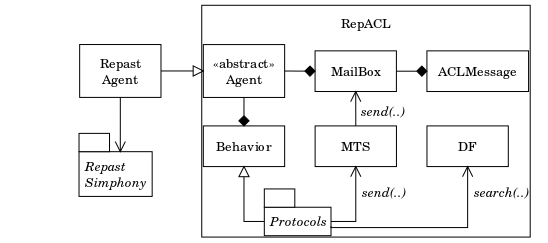
\includegraphics[width=3.5in]{figures/repacl_arch.pdf}
	\caption{Detailed architecture or \apiname{}}
	\label{fig:arch}
\end{figure}



% section proposal (end)